\documentclass[a4paper,11pt,exos]{nsi} % COMPILE WITH DRAFT
\usepackage{pifont}
\usepackage{fontawesome5}
\usepackage{hyperref}



\begin{document}
\classe{\terminale Comp}
\titre{Corrigé des exercices - Fonction $\ln$}
\maketitle

\subsection*{Définition de la fonction logarithme népérien}

\exo{} %Indice p 85
\begin{enumerate}
    \item Pour quelles valeurs de $x$, $\ln(x)$ est-il défini ?
    \item Donner la valeur de $e^{\ln 7}$.
    \item Donner la valeur de $\ln(e^5)$ et de $\ln(e^{-3})$.
    \item On note $\mathcal{C}$ la courbe représentative de la fonction $\ln$ dans un repère orthonormé.\\
    Indiquer si les affirmations suivantes sont vraies ou fausses :
    \begin{enumalph}
        \item $\mathcal{C}$ est au-dessus de l'axe des abscisses.
        \item $\mathcal{C}$ passe par le point de coordonnées $(1,0)$.
    \end{enumalph}
\end{enumerate} 
\textcolor{UGLiBlue}{
    \begin{enumerate}
        \item $\ln(x)$ est défini pour $x>0$.
        \item $e^{\ln 7}=7$.
        \item $\ln(e^5)=5$ et $\ln(e^{-3})=-3$.
        \item \begin{enumalph}
            \item Faux, $\mathcal{C}$ est en-dessous de l'axe des abscisses pour sur $\oio{0}{1}$.
            \item Vrai, $\ln(1)=0$. $\mathcal{C}$ passe par le point de coordonnées $(1,0)$.
        \end{enumalph}
    \end{enumerate}
}

\exo{} %Indice p 85
Simplifier les expressions suivantes :
\begin{multicols}{3}
    \begin{enumerate}
        \item $\dfrac{\ln\left(e^{-2}\right)}{\ln\left(e^4\right)}$
        \item $\ln\left(e^9\right)\times\ln\left(e^{-2}\right)$
        \item $\ln\left(e\right)+\ln\left(\dfrac{1}{e}\right)$
        %\item $\ln\left(\dfrac{1}{e}\right)+\ln\left(\dfrac{1}{e^2}\right)$
    \end{enumerate}
\end{multicols}

\textcolor{UGLiBlue}{
    \begin{enumerate}
        \item $\dfrac{\ln\left(e^{-2}\right)}{\ln\left(e^4\right)}=\dfrac{-2}{4}=-\dfrac{1}{2}$.
        \item $\ln\left(e^9\right)\times\ln\left(e^{-2}\right)=9\times (-2)=-18$.
        \item $\ln\left(e\right)+\ln\left(\dfrac{1}{e}\right)=\ln(e^1)+\ln(e^{-1})=1+(-1)=0$.
        %\item $\ln\left(\dfrac{1}{e}\right)+\ln\left(\dfrac{1}{e^2}\right)=-1-(-2)=1$.
    \end{enumerate}
}

\exo{}
Parmi les courbes suivantes, quelle est la représentation graphique de la fonction $\ln$ ?
\begin{center}
    \def\xmin{-3} \def\ymin{-3}\def\xmax{8}\def\ymax{3}
		\begin{tikzpicture}[scale=.7]
			\clip (\xmin,\ymin) rectangle (\xmax,\ymax);
			\draw[fill = white] (\xmin,\ymin) rectangle (\xmax,\ymax);
			\repereal{\xmin}{\ymin}{\xmax}{\ymax}
			\draw[color=UGLiRed,thick,samples=1000,domain=0.01:\xmax,smooth,variable=\x] plot ({\x},{ln(\x)});
            \draw[color=UGLiBlue,thick,samples=1000,domain=-1.99:\xmax,smooth,variable=\x] plot ({\x},{ln(\x+2)});
            \draw[color=UGLiGreen,thick,samples=1000,domain=1.01:\xmax,smooth,variable=\x] plot ({\x},{ln(-1+\x)});
            \draw[color=UGLiOrange,thick,samples=1000,domain=0.01:\xmax,smooth,variable=\x] plot ({\x},{-(\x-2)^2+1});
		\end{tikzpicture}
\end{center}

\textcolor{UGLiBlue}{
    La courbe rouge est la représentation graphique de la fonction $\ln$.
}

\exo{}
Sans les calculer, déterminer le signe de chacun des nombres suivants :
\begin{multicols}{3}
    \begin{enumerate}
        \item $\ln\left(8\right)$
        \item $\ln\left(0,1\right)$
        \item $\ln\left(\dfrac{1}{6}\right)$
        \item $\ln\left(1,9\right)$
        \item $\ln\left(100\right)$
        \item $\ln\left(2\times 10^{-3}\right)$
    \end{enumerate}
\end{multicols}

\textcolor{UGLiBlue}{
    \begin{multicols}{3}
        \begin{enumerate}
            \item $\ln\left(8\right)>0$.
            \item $\ln\left(0,1\right)<0$.
            \item $\ln\left(\dfrac{1}{6}\right)<0$.
            \item $\ln\left(1,9\right)>0$.
            \item $\ln\left(100\right)>0$.
            \item $\ln\left(2\times 10^{-3}\right)<0$.
        \end{enumerate}
    \end{multicols}
}


\exo{}
Dans chaque cas, pour quelles valeurs de $x$, les expressions suivantes sont-elles définies ?
\begin{multicols}{3}
    \begin{enumerate}
        \item $\ln\left(x-5\right)$
        \item $\ln\left(6-3x\right)$
        \item $\ln\left(x\right)+\ln\left(4-x\right)$
    \end{enumerate}
\end{multicols}

\textcolor{UGLiBlue}{
    %\begin{multicols}{3}
        \begin{enumerate}
            \item $\ln\left(x-5\right)$ est défini pour $x-5>0$ soit $x>5$.
            \item $\ln\left(6-3x\right)$ est défini pour $6-3x>0$ soit $x<2$.
            \item $\ln\left(x\right)+\ln\left(4-x\right)$ est défini pour $x>0$ et $4-x>0$ soit $0<x<4$.
        \end{enumerate}
    %\end{multicols}
}

\newpage
\subsection*{Résoudre des équations et des inéquations}
\exo{}
\begin{multicols}{2}
    \begin{enumerate}
        \item On sait que $e^x=5$. Que vaut $x$ ?
        \item On sait que $\ln(x)=0$. Que vaut $x$ ?
        \item On sait que $\ln(x)=9$. Que vaut $x$ ?
        \item On sait que $\ln(x)=-3$. Que vaut $x$ ?
    \end{enumerate}
    
    \textcolor{UGLiBlue}{
        \begin{enumerate}
            \item $e^x=5$ donc $x=\ln(5)$.
            \item $\ln(x)=0$ donc $x=e^0=1$.
            \item $\ln(x)=9$ donc $x=e^9$.
            \item $\ln(x)=-3$ donc $x=e^{-3}$.
        \end{enumerate}
    }
\end{multicols}


\exo{}
Résoudre les équations suivantes dans $\oio{0}{+\infty}$ :
\begin{multicols}{4}
    \begin{enumerate}
        \item $\ln(x)=1$
        \item $\ln(x)=7$
        \item $\ln(x)=-2$
        \item $\ln(x)=-1$
    \end{enumerate}
\end{multicols}

\textcolor{UGLiBlue}{
    \begin{multicols}{2}
        \begin{enumerate}
            \item \begin{tabbing}
                $\ln(x)=1\quad$ \= $\iff \quad x=e^1$\\
                \> $\iff \quad x=e$
            \end{tabbing}
            $\mathcal{S}_1=\left\{e\right\}$
            \item \begin{tabbing}
                $\ln(x)=7\quad$ \= $\iff \quad x=e^7$
            \end{tabbing}
            $\mathcal{S}_2=\left\{e^7\right\}$
            \vfill\null
            \columnbreak
            \item \begin{tabbing}
                $\ln(x)=-2\quad$ \= $\iff \quad x=e^{-2}$\\
                \> $\iff \quad x=\dfrac{1}{e^2}$
            \end{tabbing}
            $\mathcal{S}_3=\left\{\dfrac{1}{e^2}\right\}$
            \item \begin{tabbing}
                $\ln(x)=-1\quad$ \= $\iff \quad x=e^{-1}$\\
                \> $\iff \quad x=\dfrac{1}{e}$
            \end{tabbing}
            $\mathcal{S}_4=\left\{\dfrac{1}{e}\right\}$
        \end{enumerate}
    \end{multicols}
}

\exo{}
Résoudre les équations suivantes dans $\oio{0}{+\infty}$ :
\begin{multicols}{4}
    \begin{enumerate}
        \item $\e^{x}=10$
        \item $3e^x+5=14$
        \item $\ln(2x)+1=0$
        \item $\ln(x)=\ln(2x+1)$
    \end{enumerate}
\end{multicols}

\newpage
\textcolor{UGLiBlue}{
    \begin{multicols}{2}
        \begin{enumerate}
            \item \begin{tabbing}
                $\e^{x}=10\quad$ \= $\iff \quad x=\ln(10)$
            \end{tabbing}
            $\mathcal{S}_1=\left\{\ln(10)\right\}$
            \item \begin{tabbing}
                $3e^x+5=14\quad$ \= $\iff \quad 3e^x=9$\\
                \> $\iff \quad e^x=3$\\
                \> $\iff \quad x=\ln(3)$
            \end{tabbing}
            $\mathcal{S}_2=\left\{\ln(3)\right\}$
            \vfill\null
            \columnbreak
            \item \begin{tabbing}
                $\ln(2x)+1=0\quad$ \= $\iff \quad \ln(2x)=-1$\\
                \> $\iff \quad 2x=e^{-1}$\\
                \> $\iff \quad x=\dfrac{1}{2e}$
            \end{tabbing}
            $\mathcal{S}_3=\left\{\dfrac{1}{2e}\right\}$
            \item \begin{tabbing}
                $\ln(x)=\ln(2x+1)\quad$ \= $\iff \quad x=2x+1$\\
                \> $\iff \quad x=-1$
            \end{tabbing}
            $\mathcal{S}_4=\left\{-1\right\}$
        \end{enumerate}
    \end{multicols}
}

\exo{}
Dans chaque cas, déterminer l'ensemble des nombres réels $x$ pour lesquels les expressions sont bien définies puis résoudre l'inéquation :
\begin{multicols}{4}
    \begin{enumerate}
        \item $\ln(x)\leqslant 2$
        \item $\ln(3x)\geqslant \ln(6)$
        \item $\ln(1-x)> 0$
        \item $\ln(3-2x)\leqslant 1$
        \item $\ln(x-4)\leqslant \ln(1+2x)$
        \item $\ln(x^2-9)>\ln(2)$
        \item $3e^x-1<8$
        \item $e^{2x}-3e^x\geqslant 0$
    \end{enumerate}
\end{multicols}

\textcolor{UGLiBlue}{
    %\begin{multicols}{2}
        \begin{enumerate}
            \item $\ln(x)$ est bien défini pour $x>0$.
            \begin{tabbing}
                $\ln(x)\leqslant 2\quad$ \= $\iff \quad x\leqslant e^2$
            \end{tabbing}
            $\mathcal{S}_1=\oif{0}{e^2}$
            \item $\ln(3x)$ est bien défini pour $3x>0$ soit $x>0$.
            \begin{tabbing}
                $\ln(3x)\geqslant \ln(6)\quad$ \= $\iff \quad 3x\geqslant 6$\\
                \> $\iff \quad x\geqslant 2$
            \end{tabbing}
            $\mathcal{S}_2=\fio{2}{+\infty}$
            \item $\ln(1-x)$ est bien défini pour $1-x>0$ soit $x<1$.
            \begin{tabbing}
                $\ln(1-x)> 0\quad$ \= $\iff \quad \ln(1-x)>\ln(1)$\\
                \> $\iff \quad 1-x>1$\\
                \> $\iff \quad x<2$
            \end{tabbing}
            $\mathcal{S}_3=\oio{0}{1}$
            \item $\ln(3-2x)$ est bien défini pour $3-2x>0$ soit $x<\dfrac{3}{2}$.
            \begin{tabbing}
                $\ln(3-2x)\leqslant 1\quad$ \= $\iff \quad \ln(3-2x)\leqslant \ln(e)$\\
                \> $\iff \quad 3-2x\leqslant e$\\
                \> $\iff \quad x\geqslant \dfrac{3-e}{2}$
            \end{tabbing}
            $\mathcal{S}_4=\fio{\dfrac{3-e}{2}}{\dfrac{3}{2}}$
            \item $\ln(x-4)$ est bien défini pour $x-4>0$ soit $x>4$.\\
            $\ln(1+2x)$ est bien défini pour $1+2x>0$ soit $x>-\dfrac{1}{2}$.\\
            Les deux expressions sont donc bien définies pour $x>4$.
            \begin{tabbing}
                $\ln(x-4)\leqslant \ln(1+2x)\quad$ \= $\iff \quad x-4\leqslant 1+2x$\\
                \> $\iff \quad -4\leqslant 1+x$\\
                \> $\iff \quad x\geqslant -5$
            \end{tabbing}
            $\mathcal{S}_5=\oio{4}{+\infty}$
            \item $\ln(x^2-9)$ est bien défini pour $x^2-9>0$ soit $x\in\left]-\infty;-3\right[\cup\left]3;+\infty\right[$.
            \begin{tabbing}
                $\ln(x^2-9)>\ln(2)\quad$ \= $\iff \quad x^2-9>2$\\
                \> $\iff \quad x^2>11$\\
                \> $\iff \quad x\in\left]-\infty;-\sqrt{11}\right[\cup\left]\sqrt{11};+\infty\right[$
            \end{tabbing}
            $\mathcal{S}_6=\left]-\infty;-\sqrt{11}\right[\cup\left]\sqrt{11};+\infty\right[$
            \item $3e^x-1$ est bien défini pour tout $x\in\mathbb{R}$.
            \begin{tabbing}
                $3e^x-1<8\quad$ \= $\iff \quad 3e^x<9$\\
                \> $\iff \quad e^x<3$\\
                \> $\iff \quad x<\ln(3)$
            \end{tabbing}
            $\mathcal{S}_7=\oio{-\infty}{\ln(3)}$
            \item $e^{2x}-3e^x$ est bien défini pour tout $x\in\mathbb{R}$.
            \begin{tabbing}
                $e^{2x}-3e^x\geqslant 0\quad$ \= $\iff \quad e^{2x}\geqslant 3e^x$\\
                \> $\iff \quad e^x\times e^x\geqslant 3e^x$\\
                \> $\iff \quad e^x\geqslant 3$\\
                \> $\iff \quad x\geqslant \ln 3$
            \end{tabbing}
            $\mathcal{S}_8=\fio{\ln 3}{+\infty}$
        \end{enumerate}
    %\end{multicols}
}


\exo{ \faStar}
On veut résoudre l'équation $\quad e^{2x}-2e^x=8\ (E)$.
\begin{enumerate}
    \item On pose $y=e^x$. Montrer que l'équation précédente est équivalente à $y^2-2y-8=0\ (E')$.
    \item Résoudre l'équation $(E')$.
    \item En déduire les solutions de l'équation initiale $(E)$.
\end{enumerate}

\newpage
\textcolor{UGLiBlue}{
    \begin{enumerate}
        \item Soit $x\in\R$.
        \begin{tabbing}
            $e^{2x}-2e^x=8\quad$ \= $\iff \quad e^x\times e^x-2e^x=8$\\
            \> $\iff \quad \left(e^x\right)^2-2e^x-8=0$\\
            \>$\iff \quad y^2-2y-8=0$
        \end{tabbing}
        \item $y^2-2y-8=0$ est une équation du second degré.\\[.5em]
        $\Delta=4+32=36\quad$ et $\quad y_1=\dfrac{2+6}{2}=4\quad$ et $\quad y_2=\dfrac{2-6}{2}=-2$.\\[.5em]
        Les solutions de l'équation $(E')$ sont $y_1=4$ et $y_2=-2$.
        \item \begin{tabbing}
            $e^{2x}-2e^x=8\quad$ \= $\iff \quad e^x=4\quad$ ou $\quad \underbrace{e^x=-2}_{\text{impossible}}$\\
            \> $\iff \quad x=\ln 4\quad $
        \end{tabbing}
        L'équation $(E)$ a donc une seule solution : $\ln 4$.
    \end{enumerate}
}

\subsection*{Propriétés algébriques du logarithme népérien}
\exo{}
Exprimer les nombres suivants en fonction de $\ln 2$.
\begin{multicols}{4}
    \begin{enumerate}
        \item $\ln 4$
        \item $\ln 8$
        %\item $\ln 16$
        \item $\ln \dfrac{1}{2}$
        \item $\ln \dfrac{1}{8}$
        \item $\ln (8e)$
        \item $\ln \left(4e^2\right)$
        \item $\ln \sqrt{2}$
        \item $\ln \sqrt{32}$
    \end{enumerate}
\end{multicols}

\textcolor{UGLiBlue}{
    \begin{multicols}{2}
        \begin{enumerate}
            \item $\ln 4=2\ln 2$
            \item $\ln 8=3\ln 2$
            %\item $\ln 16=4\ln 2$
            \item $\ln \dfrac{1}{2}=-\ln 2$
            \item $\ln \dfrac{1}{8}=-3\ln 2$
            \item $\ln (8e)=\ln 8+\ln e=3\ln 2+1$
            \item $\ln \left(4e^2\right)=\ln 4+\ln e^2=2\ln 2+2$
            \item $\ln \sqrt{2}=\dfrac{1}{2}\ln 2$
            \item $\ln \sqrt{32}=\dfrac{1}{2}\ln 32=\dfrac{1}{2}\times 5\ln 2=\dfrac{5}{2}\ln 2$
        \end{enumerate}
    \end{multicols}
}

\exo{}
Écrire les nombres suivants en utilisant une seule fois le symbole $\ln$.
\begin{multicols}{2}
    \begin{enumerate}
        \item $A= 5\ln 2+\ln 8-\ln 4$
        \item $B=2\ln 3+\ln 81-\ln 9$
        \item $C=\ln 3-\ln 2+\ln 5$
        \item $D=\ln 14-\ln 19$
    \end{enumerate}
\end{multicols}

\textcolor{UGLiBlue}{
    \begin{multicols}{2}
        \begin{enumerate}
            \item \begin{tabbing}
                $A$ \= $=5\ln 2+\ln 8-\ln 4$\\
                \>$=5\ln 2+\ln 2^3-\ln 2^2$\\
                \>$=5\ln 2+3\ln 2-2\ln 2$\\
                \>$=6\ln 2$
            \end{tabbing}
            \item \begin{tabbing}
                $B$ \= $=2\ln 3+\ln 81-\ln 9$\\
                \>$=2\ln 3+\ln 3^4-\ln 3^2$\\
                \>$=2\ln 3+4\ln 3-2\ln 3$\\
                \>$=4\ln 3$
            \end{tabbing}
            \columnbreak
            \item \begin{tabbing}
                $C$ \= $\ln 3-\ln 2+\ln 5$\\
                \> $=\ln \dfrac{3\times 5}{2}$\\
                \> $=\ln \dfrac{15}{2}$
            \end{tabbing}
            \item \begin{tabbing}
                $D$ \= $\ln 14-\ln 19$\\
                \> $=\ln \dfrac{14}{19}$
            \end{tabbing}
        \end{enumerate}
    \end{multicols}
}

\exo{}
\begin{enumerate}
    \item Écrire le réel $\ln 7 +\ln 2$ en utilisant une seule fois le symbole $\ln$.
    \item En déduire les solution de l'équation $\ln x=\ln 7 +\ln 2$ dans $\oio{0}{+\infty}$.
\end{enumerate}

\textcolor{UGLiBlue}{
    \begin{enumerate}
        \item $\ln 7 +\ln 2=\ln(2\times 7)=\ln 14$.
        \item \begin{tabbing}
            $\ln x=\ln 7 +\ln 2\quad$ \= $\iff \quad \ln x=\ln 14$\\
            \> $\iff \quad x=14$
        \end{tabbing}
        Donc l'équation $\ln x=\ln 7 +\ln 2$ a une seule solution dans $\oio{0}{+\infty}$ : $14$.
    \end{enumerate}
}

\exo{}
On considère l'équation $(E) : \ln(x)+ \ln(2x)=\ln(18)$ pour $x$ appartenant à $\oio{0}{+\infty}$.
\begin{enumerate}
    \item Montrer que l'équation $(E)$ est équivalente à $x^2=9$ pour $x>0$.
    \item En déduire l'ensemble des solutions de l'équation $(E)$.
\end{enumerate}

\textcolor{UGLiBlue}{
    \begin{enumerate}
        \item Soit $x>0$.
        \begin{tabbing}
            $\ln(x)+ \ln(2x)=\ln(18)\quad$ \= $\iff \quad \ln(x\times 2x)=\ln(18)$\\
            \> $\iff \quad \ln(2x^2)=\ln(18)$\\
            \> $\iff \quad 2x^2=18$\\
            \> $\iff \quad x^2=9$
        \end{tabbing}
        \item Les solutions de l'équation $(E)$ dans $\R$ sont $3$ et $-3$.\\
        Seule la solution $3$ appartient à $\oio{0}{+\infty}$ donc l'équation $(E)$ admet une seule solution dans $\oio{0}{+\infty}$ : $3$.
    \end{enumerate}
}

\exo{ \faStar}
On veut résoudre l'équation $\quad \left(\ln x\right)^2+4\ln \dfrac{1}{x}-5=0\ (E)$.
\begin{enumerate}
    \item On pose $y=\ln x$. Montrer que l'équation précédente est équivalente à $y^2-4y-5=0\ (E')$.
    \item Résoudre l'équation $(E')$.
    \item En déduire les solutions de l'équation initiale $(E)$.
\end{enumerate}

\textcolor{UGLiBlue}{
    \begin{enumerate}
        \item Soit $x>0$.
        \begin{tabbing}
            $\left(\ln x\right)^2+4\ln \dfrac{1}{x}-5=0\quad$ \= $\iff \quad \left(\ln x\right)^2+4(-\ln x)-5=0$\\
            \> $\iff \quad y^2+4(-y)-5=0$\\
            \> $\iff \quad y^2-4y-5=0$
        \end{tabbing}
        \item $y^2-4y-5=0$ est une équation du second degré.\\[.5em]
        $\Delta=16+20=36\quad$ et $\quad y_1=\dfrac{4+6}{2}=5\quad$ et $\quad y_2=\dfrac{4-6}{2}=-1$.\\[.5em]
        Les solutions de l'équation $(E')$ sont $y_1=5$ et $y_2=-1$.
        \item \begin{tabbing}
            $\left(\ln x\right)^2+4\ln \dfrac{1}{x}-5=0\quad$ \= $\iff\quad \ln x=5\quad$ ou $\quad \ln x=-1$\\
            \>$\iff \quad x=e^5\quad$ ou $\quad x=e^{-1}$
        \end{tabbing}
        Les solutions de l'équation $(E)$ sont $e^5$ et $e^{-1}$.
    \end{enumerate}
}

\exo{}
Dans chaque cas, utiliser la fonction logarithme népérien pour résoudre les équations suivantes dans $\oio{0}{+\infty}$ :
\begin{multicols}{3}
    \begin{enumerate}
        \item $x^5=100$
        \item $x^7=42$
        \item $x^6=1,5$
    \end{enumerate}
\end{multicols}

\textcolor{UGLiBlue}{
    \begin{multicols}{2}
        \begin{enumerate}
            \item \begin{tabbing}
                $x^5=100\quad$ \= $\iff \quad \ln\left(x^5\right)=\ln 100$\\
                \> $\iff \quad 5\ln x=\ln 100$\\
                \> $\iff \quad \ln x=\dfrac{1}{5}\ln 100$\\[.5em]
                \> $\iff \quad x=e^{\frac{1}{5}\ln 100}$
            \end{tabbing}
            \item \begin{tabbing}
                $x^7=42\quad$ \= $\iff \quad \ln x^7=\ln 42$\\
                \> $\iff \quad 7\ln x=\ln 42$\\
                \> $\iff \quad \ln x=\dfrac{1}{7}\ln 42$\\[.5em]
                \> $\iff \quad x=e^{\frac{1}{7}\ln 42}$
            \end{tabbing}
            \item \begin{tabbing}
                $x^6=1,5\quad$ \= $\iff \quad \ln x^6=\ln 1,5$\\
                \> $\iff \quad 6\ln x=\ln 1,5$\\
                \> $\iff \quad \ln x=\dfrac{1}{6}\ln 1,5$\\[.5em]
                \> $\iff \quad x=e^{\frac{1}{6}\ln 1,5}$
            \end{tabbing}
        \end{enumerate}
    \end{multicols}
}

\exo{}
$(u_n)$ est la suite géométrique de premier terme $u_0=4$ et de raison $1,5$.
\begin{enumerate}
    \item Pour tout entier naturel $n$, exprimer $u_n$ en fonction de $n$.
    \item Calculer la limite de la suite $(u_n)$.
    \item Déterminer par le calcul le rang $n$ à partir duquel $u_n>1000$.
\end{enumerate}

\textcolor{UGLiBlue}{
\begin{enumerate}
    \item $u_n=u_0\times q^n=4\times 1,5^n$.
    \item $4>0$ et $q=1,5>1$ donc $\quad \lim\limits_{n\to+\infty}u_n=+\infty$.
    \item \begin{tabbing}
        $u_n>1000\quad$ \= $\iff \quad 4\times 1,5^n>1000$\\
        \>  $\iff \quad 1,5^n>250$\\
        \>  $\iff \quad \ln 1,5^n >\ln 250$\\
        \>  $\iff \quad n\ln 1,5 >\ln 250$\\
        \>  $\iff \quad n>\dfrac{\ln 250}{\ln 1,5}$\\
        \>  $\iff \quad n\geqslant 14$
    \end{tabbing}
    $(u_n)$ dépasse $1000$ à partir du rang $14$.
\end{enumerate}}


\exo{}
$(v_n)$ est la suite géométrique de premier terme $v_0=100$ et de raison $0,86$.
\begin{enumerate}
    \item Pour tout entier naturel $n$, exprimer $v_n$ en fonction de $n$.
    \item Calculer la limite de la suite $(v_n)$.
    \item Déterminer par le calcul le rang $n$ à partir duquel $v_n<10^{-3}$.
\end{enumerate}

\textcolor{UGLiBlue}{
\begin{enumerate}
    \item $v_n=v_0\times q^n=100\times 0,86^n$.
    \item $q=0,86<1$ donc $\quad \lim\limits_{n\to+\infty}v_n=0$.
    \item \begin{tabbing}
        $v_n<10^{-3}\quad$ \= $\iff \quad 100\times 0,86^n<10^{-3}$\\
        \>  $\iff \quad 0,86^n<10^{-5}$\\
        \>  $\iff \quad \ln 0,86^n <\ln 10^{-5}$\\
        \>  $\iff \quad n\ln 0,86 <\ln 10^{-5}$\\
        \>  $\iff \quad n>\dfrac{\ln 10^{-5}}{\ln 0,86} \qquad$ car $\ln 0,86 <0$.\\
        \>  $\iff \quad n\geqslant 77$
    \end{tabbing}
    $(v_n)$ devient inférieure à $10^{-3}$ à partir du rang $77$.
\end{enumerate}}

\exo{}
Une infographiste simule la croissance d'un bambou d'une taille initiale de 1 m.\\
Pour tout entier naturel $n\geqslant 1$, on modélise la taille, en cm, qu'aurait le bambou à la fin du $n$-ième mois par la suite $(u_n)$ définie par $u_n=500\times 1,5^n-400$.
\begin{enumerate}
    \item Calculer la taille, en cm, du bambou à la fin du 3$^{\text{e}}$ mois. Arrondir au dixième.
    \item Résoudre dans $\N$ l'inéquation $u_n>300$. Interpréter le résultat dans le contexte de l'exercice.
    \item Déterminer, en résolvant une inéquation, le nombre de mois nécessaires pour que le bambou dépasse 10 m.
\end{enumerate}

\textcolor{UGLiBlue}{
    \begin{enumerate}
        \item \begin{tabbing}
            $u_3$\=$=500\times 1,5^3-400$\\
            \> $=500\times 3,375-400$\\
            \> $=1687,5-400$\\
            \> $=1287,5$ cm
        \end{tabbing}
        La taille du bambou à la fin du 3$^{\text{e}}$ mois est de 1287,5 cm.
        \item \begin{tabbing}
            $u_n>300$ \= $\iff \quad 500\times 1,5^n-400>300$\\
            \> $\iff \quad 500\times 1,5^n>700$\\
            \> $\iff \quad 1,5^n>\dfrac{700}{500}$\\
            \> $\iff \quad 1,5^n>1,4$\\
            \> $\iff \quad \ln 1,5^n>\ln 1,4$\\
            \> $\iff \quad n\ln 1,5>\ln 1,4$\\
            \> $\iff \quad n>\dfrac{\ln 1,4}{\ln 1,5}$\\
            \> $\iff \quad n\geqslant 1$
        \end{tabbing}
        Le bambou mesure plus de 3 m à partir du 1$^{\text{er}}$ mois.
        \item \begin{tabbing}
            $u_n>1000$ \= $\iff \quad 500\times 1,5^n-400>1000$\\
            \> $\iff \quad 500\times 1,5^n>1400$\\
            \> $\iff \quad 1,5^n>\dfrac{1400}{500}$\\
            \> $\iff \quad 1,5^n>2,8$\\
            \> $\iff \quad \ln 1,5^n>\ln 2,8$\\
            \> $\iff \quad n\ln 1,5>\ln 2,8$\\
            \> $\iff \quad n>\dfrac{\ln 2,8}{\ln 1,5}$\\
            \> $\iff \quad n\geqslant 3$
        \end{tabbing}
        Le bambou mesure plus de 10 m à partir du 3$^{\text{e}}$ mois.
    \end{enumerate}}

%\newpage

\exo{}
%exercice 123 p 106 hyperbole
Le carbone 14 (C$_{14}$) présent dans l'organisme d'un être vivant se désintègre au fil des années après sa mort. Le nombre d'années $N$ nécessaires à l'observation de la proportion $p$ de C$_{14}$ restante dans l'organisme peut être modélisé par : $N=-8310 \ln p$.
\begin{enumerate}
    \item Le squelette d'un homme de Cro-Magnon contient 9 \% de C$_{14}$ par rapport à un squelette vivant. Combien d'années se sont écoulées depuis sa mort ?

    \dleft{14cm}{\item Lucy est la plus ancienne hominidé connue. Les paléontologues estiment à au moins 3,5 millions d'années son âge. A-t-on pu dater les fragments de son squelette à l'aide du carbone 14 ? Justifier.}{\includegraphics[width=1.8cm]{Lucy.jpg}}
    \dleft{13cm}{\item Découverte en 1991 en Italie, la momie d'Ötzi contenait 53,3 \% (à 1\% près) de C$_{14}$ par rapport à un homme vivant. Donner un encadrement de l'âge d'Ötzi.}
    {\includegraphics[width=2.8cm]{Otzi-Quinson.jpg}}
\end{enumerate}

\textcolor{UGLiBlue}{
    \begin{enumerate}
        \item \begin{tabbing}
            $N=-8310 \ln p\quad$ \= $\iff \quad N=-8310 \ln 0,09$\\
            \> $\iff \quad N\approx 20\ 010$
        \end{tabbing}
        Le squelette de l'homme de Cro-Magnon date d'environ 20 000 ans.
        \item \begin{tabbing}
            $N=-8310 \ln p\quad$ \= $\iff \quad 3,5 \times 10^6=-8310 \ln p$\\
            \> $\iff \quad \ln p= -\dfrac{3,5\times 10^6}{8310}$\\[.5em]
            \> $\iff \quad p=e^{-\dfrac{3,5\times 10^6}{8310}}$\\
            \> $\iff \quad p\approx 10^{-183}$
        \end{tabbing}
        La proportion de C$_{14}$ restante dans le squelette est de l'ordre de $10^{-183}$, ce qui est extrèmement faible. On ne peut donc pas dater les fragments de son squelette à l'aide du carbone 14.
        \item \begin{tabbing}
            $0,523<p<0,543 \quad$ \= $\iff \quad  \ln 0,523<\ln p<\ln 0,543$\\
            \> $\iff \quad -8310\times\ln 0,523>-8310 \ln p >-8310\times \ln 0,543$\\
            \> $\iff \quad 5387>N>5074$
        \end{tabbing}
        L'âge d'Ötzi est compris entre 5074 et 5387 ans.
    \end{enumerate}
}

\exo{}
\dleft{12cm}{
    Dans une réserve marine, on a recencé 3000 cétacés au 1$^{\text{er}}$ janvier 2020. Les responsables sont inquiets car le classement de la zone en « réserve marine » ne sera pas reconduit si le nombre de cétacés de cette réserve devient inférieur à 2000.\\
    Une étude permet d'élaborer un nodèle selon lequel :
}
{\includegraphics[width=4.2cm]{whale-4424846_1280.jpg}}
\begin{enumerate}[label=\textbullet]
    \item entre le 1$^{\text{er}}$ juin et le 31 octobre, 80 cétacés arrivent dans la réserve marine ;
    \item entre le 1$^{\text{er}}$ novembre et le 31 mai, la réserve subit une baisse de 5 \% de son effectif par rapport à celui du 31 octobre.
\end{enumerate}
On modélise le nombre de cétacés dans la réserve marine au 1$^{\text{er}}$ juin de l'année 2020 $+n$ par le terme $u_n$. Ainsi $u_0=3000$.
\begin{enumerate}
    \item Justifier que $u_1=2926$.
    \item Justifier que pour tout $n\in\N$, $u_{n+1}=0,95u_n+76$.
    \item Démontrer que pour tout $n\in\N$, $u_{n}=1480\times 0,95^n+1520$.
    \item Déterminer la limite de la suite $(u_n)$.
    \item La réserve marine fermera-elle ? Si oui, en quelle année ? \textit{Répondre à l'aide d'un calcul.}
\end{enumerate}

\textcolor{UGLiBlue}{
    \begin{enumerate}
        \item $u_1=0,95\times (3000+80)=2926$.
        \item Soit $n\in\N$.
        \begin{tabbing}
            $u_{n+1}$ \= $=0,95\times (u_n+80)$\\
            \> $=0,95\times u_n+0,95\times 80$\\
            \> $=0,95\times u_n+76$
        \end{tabbing}
        \item On a pour tout $n\in\N, u_{n+1}=0,95 u_n+76$ et $u_0=3000$.\\
        $(u_n)$ est une suite arithmétique de premier terme $u_0=3000$ et de raison $q=0,95$.\\[.5em]
        \textbf{Suite constante vérifiant la relation de récurrence :} \begin{tabbing}
            Soit $x\in\R \qquad x=0,95x+76$\=$\iff x-0,95x=76$\\
            \>$\iff 0,05x=76$\\
            \>$\iff x=1520$.
        \end{tabbing}
        La suite constante $(c_n)$ égale à 1520 vérifie donc la relation $c_{n+1}=0,95c_n+76$ pour tout $n\in\N$.\\[.5em]
        \textbf{Suite géométrique auxiliaire :}\\[.5em]
        On définit la suite $(v_n)$ sur $\N$ par $v_n=t_n-c_n$.\\
        Montrons que $(v_n)$ est une suite géométrique :
        \begin{tabbing}
            Soit $n\in\N \qquad v_{n+1}$\=$=u_{n+1}-c_{n+1}$\\
            \> $=0,95u_n+76-(0,95c_n+76)$\\
            \> $=0,95u_n+76-0,95c_n-76$\\
            \> $=0,95(u_n-c_n)$\\
            \> $=0,95v_n$.
        \end{tabbing}
        $(v_n)$ est donc une suite géométrique de raison $q=0,95$ et de premier terme $v_0=u_0-c_0=3000-1520=1480$.\\
        On a donc pour tout $n\in\N, v_n=v_0\times 0,95^n=1480\times 0,95^n$.\\[.5em]
        \textbf{Terme général de la suite $(u_n)$ :}\\[.5em]
        On a donc pour tout $n\in\N, u_n=c_n+v_n=1520+1480\times 0,95^n$.
        \item $0<0,95<1$ donc $\lim\limits_{n\to+\infty}u_n=1520$.
        \item \begin{tabbing}
            $u_n<2000\quad$ \= $\iff \quad 1520+1480\times 0,95^n<2000$\\
            \> $\iff \quad 1480\times 0,95^n<480$\\
            \> $\iff \quad 0,95^n<\dfrac{480}{1480}$\\[.5em]
            \> $\iff \quad 0,95^n<\dfrac{12}{37}$\\[.5em]
            \> $\iff \quad \ln 0,95^n<\ln \dfrac{12}{37}$\\[.5em]
            \> $\iff \quad n\ln 0,95<\ln \dfrac{12}{37}$\\[.5em]
            \> $\iff \quad n>\dfrac{\ln \dfrac{12}{37}}{\ln 0,95}$\\[.5em]
            \> $\iff \quad n\geqslant 22$
        \end{tabbing}
        La réserve marine fermera donc à partir de l'année 2042.
    \end{enumerate}
}

%\newpage

\exo{}
Une agence bancaire propose un placement à tous ses clients. Ce placement a rapporté 30 \% d'intérêts sur les 5 dernières années.\\
On note $t$ \% le taux d'intérêt annuel moyen de ce placement sur ces 5 dernières années.
\begin{enumerate}
    \item Justifier que le taux d'intérêt annuel moyen $t$ est tel que $1,3=\left(1+\dfrac{t}{100}\right)^5$.
    \item Résoudre l'équation précédente en utilisant la fonction logarithme népérien. \textit{Donner la valeur exacte, puis l'arrondi au centième.}
    \item Interpréter le résultat obtenu dans le contexte de la situation.
\end{enumerate}

\textcolor{UGLiBlue}{
    \begin{enumerate}
        \item Soit $t$ le taux d'intérêt annuel moyen de ce placement sur ces 5 dernières années.\\
        Chaque année, le montant du placement est multiplié par $1+\dfrac{t}{100}$.\\
        Après 5 ans, le montant du placement est multiplié par $\left(1+\dfrac{t}{100}\right)^5$.\\
        On a donc $\left(1+\dfrac{t}{100}\right)^5=1+\dfrac{30}{100}=1,3$.
        \item \begin{tabbing}
            $\left(1+\dfrac{t}{100}\right)^5=1,3\quad$ \= $\iff \quad \ln\left(\left(1+\dfrac{t}{100}\right)^5\right)=\ln 1,3$\\
            \> $\iff \quad 5\ln\left(1+\dfrac{t}{100}\right)=\ln 1,3$\\
            \> $\iff \quad \ln\left(1+\dfrac{t}{100}\right)=\dfrac{\ln 1,3}{5}$\\
            \> $\iff \quad 1+\dfrac{t}{100}=e^{\dfrac{\ln 1,3}{5}}$\\
            \> $\iff \quad \dfrac{t}{100}=e^{\dfrac{\ln 1,3}{5}}-1$\\
            \> $\iff \quad t=100\times\left(e^{\dfrac{\ln 1,3}{5}}-1\right)$\\
            \> $\iff \quad t\approx 5,39$
        \end{tabbing}
        \item Le taux d'intérêt annuel moyen de ce placement sur ces 5 dernières années est de 5,39\%.\\
        Ce placement a donc rapporté en moyenne 5,39\% d'intérêts par an sur les 5 dernières années.
    \end{enumerate}
}

\subsection*{Étude de la fonction logarithme népérien}

\exo{}
Dans chaque cas, donner la fonction dérivée de la fonction $f$ définie sur $\oio{0}{+\infty}$.
\begin{multicols}{3}
    \begin{enumerate}
        \item $f(x)=5\ln(x)$
        \item $f(x)=3-2\ln(x)$
        \item $f(x)=x\ln\left(x\right)-1$
        \item $f(x)=\ln(2x)$
        \item $f(x)=\ln\left(x^2\right)$
        \item $f(x)=\ln\left(3x^2+1\right)$
    \end{enumerate}
\end{multicols}

\textcolor{UGLiBlue}{
    \begin{multicols}{3}
        \begin{enumerate}
            \item \begin{tabbing}
                $f'(x)$\=$=5\times \dfrac{1}{x}$\\[.5em]
                \>$=\dfrac{5}{x}$
            \end{tabbing}
            \item \begin{tabbing}
                $f'(x)$\=$=-2\times \dfrac{1}{x}$\\[.5em]
                \>$=-\dfrac{2}{x}$
            \end{tabbing}
            \item \begin{tabbing}
                $f'(x)$\=$=\ln\left(x\right)+x\times \dfrac{1}{x}$\\[.5em]
                \>$=\ln(x)+1$
            \end{tabbing}
            \item \begin{tabbing}
                $f'(x)$\=$=\dfrac{2}{2x}$\\[.5em]
                \>$=\dfrac{1}{x}$
            \end{tabbing}
            \item \begin{tabbing}
                $f'(x)$\=$=\dfrac{2x}{x^2}$\\[.5em]
                \>$=\dfrac{2}{x}$
            \end{tabbing}
            \item \begin{tabbing}
                $f'(x)$\=$=\dfrac{3\times 2x}{3x^2+1}$\\[.5em]
                \>$=\dfrac{6x}{3x^2+1}$
            \end{tabbing}
        \end{enumerate}
    \end{multicols}
}

\exo{}
Soit $f$ la fonction définie sur $\oio{0}{+\infty}$ par $f(x)=\ln x +x$.
\begin{enumerate}
    \item Déterminer les limites de $f$ aux bornes de son ensemble de définition.
    \item Calculer la dérivée de $f$ et dresser le tableau de variation de $f$ sur $\oio{0}{+\infty}$.
\end{enumerate}

\textcolor{UGLiBlue}{
    \begin{multicols}{2}
        \begin{enumerate}
            \item $\lim\limits_{x\to 0} \ln x=-\infty\quad$ et $\quad\lim\limits_{x\to 0} x=0$.\\[.5em]
            D'où $\lim\limits_{x\to 0} f(x)=-\infty$.\\[1em]
            $\lim\limits_{x\to +\infty} \ln x=+\infty\quad$ et $\quad\lim\limits_{x\to +\infty} x=+\infty$.\\[.5em]
            D'où $\lim\limits_{x\to +\infty} f(x)=+\infty$.
            \item \begin{tabbing}
                $f'(x)$\=$=\dfrac{1}{x}+1$\\[.5em]
                \>$=\dfrac{x+1}{x}>0$
            \end{tabbing}
            \vfill\null
            \columnbreak
            On a donc le tableau de variations suivant :
            \begin{center}
                \begin{tikzpicture}
                    \tkzTabInit{$x$ / .7 , $f'(x)$ / .7,$f$ /2}{$0$, $+\infty$}
                    \tkzTabLine{, +,}
                    \tkzTabVar{-/$-\infty$ , +/$+\infty$}
                \end{tikzpicture}
            \end{center}
        \end{enumerate}
    \end{multicols}
}

\exo{}
Soit $f$ la fonction définie sur $\oio{0}{+\infty}$ par $f(x)=-\dfrac{1}{x}+\ln x$.
\begin{enumerate}
    \item Déterminer les limites de $f$ aux bornes de son ensemble de définition.
    \item Calculer la dérivée de $f$, en déduire son sens de variation sur $\oio{0}{+\infty}$ et son signe.
\end{enumerate}

\textcolor{UGLiBlue}{
    \begin{multicols}{2}
        \begin{enumerate}
            \item $\lim\limits_{x\to 0} -\dfrac{1}{x}=-\infty\quad$ et $\quad\lim\limits_{x\to 0} \ln x=-\infty$.\\[.5em]
            D'où $\lim\limits_{x\to 0} f(x)=-\infty$.\\[1em]
            $\lim\limits_{x\to +\infty} -\dfrac{1}{x}=0\quad$ et $\quad\lim\limits_{x\to +\infty} \ln x=+\infty$.\\[.5em]
            D'où $\lim\limits_{x\to +\infty} f(x)=+\infty$.
            \item \begin{tabbing}
                $f'(x)$\=$=\dfrac{1}{x^2}+\dfrac{1}{x}$\\[.5em]
                \>$=\dfrac{x+1}{x^2}>0$
            \end{tabbing}
            \vfill\null
            \columnbreak
            On a donc le tableau de variations suivant :
            \begin{center}
                \begin{tikzpicture}
                    \tkzTabInit{$x$ / .7 , $f'(x)$ / .7,$f$ /2}{$0$, $+\infty$}
                    \tkzTabLine{, +,}
                    \tkzTabVar{-/$-\infty$ , +/$+\infty$}
                \end{tikzpicture}
            \end{center}
        \end{enumerate}
    \end{multicols}
}

%\newpage

\exo{}
Soit $f$ la fonction définie sur $\oio{0}{14}$ par $f(x)=2-\ln \left(\dfrac{x}{2}\right)$.\\[.5em]
La courbe représentative $\mathcal{C}_f$ de la fonction $f$ est donnée dans le repère orthonormé ci-dessous.
\begin{center}
    \def\xmin{-1} \def\ymin{-1}\def\xmax{15}\def\ymax{5}
        \begin{tikzpicture}[scale=.7]
            \clip (\xmin,\ymin) rectangle (\xmax,\ymax);
            \draw[fill = white] (\xmin,\ymin) rectangle (\xmax,\ymax);
            \coordinate (M) at (1.7,2.16);
            \draw[UGLiOrange] (M) node[above]{$M$};
            \fill[UGLiOrange] (0,0) -- (1.7,0) -- (M) -- (0,2.16) ;
            \draw[UGLiOrange] (1.7,0) node[below]{$P$};
            \draw[UGLiOrange] (0,2.16) node[left]{$Q$};
            \repereal{\xmin}{\ymin}{\xmax}{\ymax}
            \draw[color=UGLiRed,thick,samples=1000,domain=0.01:14,smooth,variable=\x] plot ({\x},{2-ln(\x/2)});
            
            
        \end{tikzpicture}
\end{center}
À tout point $M$ appartenant à $\mathcal{C}_f$, on associe le point $P$ projeté orthogonal de $M$ sur l'axe des abscisses et le point $Q$ projeté orthogonal de $M$ sur l'axe des ordonnées.
\begin{enumerate}
    \item Montrer que la fonction $g:x\mapsto 2x-x\ln \left(\dfrac{x}{2}\right)$ modélise l'aire du rectangle $OPMQ$.
    \item Dresser le tableau de variation de $g$ sur $\oio{0}{14}$.
    \item En déduire les coordonnées du point $M$ pour lesquelles l'aire du rectangle $OPMQ$ est maximale.
    On admettra que $\lim\limits_{x\to 0^+} g(x)=0$.
\end{enumerate}

\exo{}%Hyperbole p 113
\dleft{12cm}{
\begin{encadrecolore}{Un peu d'histoire}{UGLiDarkBlue}
    Durant la Renaissance, le commerce se développant, les marchands ont été amenés à constituer des tables d'intérêts pour faciliter les calculs financiers. \textbf{Luca Pacioli} (1445-1517), religieux franciscain, mathématicien et fondateur de la comptabilité, présente la règle des 72 en 1494 dans son ouvrage \textit{Summa de arithmetica, geometria, proportioni et proportionalità}.\\
    Cette règle est une méthode pour estimer le temps de doublement d'un capital. Luca Pacioli estime que si un capital est placé à un taux d'intérêt annuel de $t$ \% alors il faut environ $\dfrac{72}{t}$ années pour le doubler.
\end{encadrecolore}}
{\includegraphics[width=4.2cm]{Pacioli.jpg}\\
\tiny{Portrait du mathématicien Luca Pacioli expliquant le théorème d'Euclide (oeuvre attribuée à Jacopo de Barbari, 1495).}}

\subsubsection*{Partie A : la règle des 72}
$t$ désigne un nombre réel strictement positif et $n$ est un nombre entier naturel non nul.
\begin{enumerate}
    \item Utiliser la règle de Pacioli pour estimer le nombre $n$ d'années nécessaires pour doubler un capital lorsqu'il est placé à un taux d'intérêts composés de :
    \begin{multicols}{3}
        \begin{enumerate}[label=\textbullet]
            \item $t=1$ \%
            \item $t=5$ \%
            \item $t=10$ \%
        \end{enumerate}
    \end{multicols}
    \item Au bout de $n$ années de placement au taux d'intérêt de $t$ \%, le capital est multiplié par $\left(1+\dfrac{t}{100}\right)^n$.
    \begin{enumalph}
        \item Dans chaque cas, déterminer, en utilisant la fonction $\ln$, le plus petit nombre entier naturel $n$ tel que $\left(1+\dfrac{t}{100}\right)^n\geqslant 2$.
        \begin{multicols}{3}
            \begin{enumerate}[label=\textbullet]
                \item $t=1$ \%
                \item $t=5$ \%
                \item $t=10$ \%
            \end{enumerate}
        \end{multicols}
        \item Comparer les résultats obtenus dans les questions 1 et 2.
    \end{enumalph}
\end{enumerate}

\subsubsection*{Partie B : une autre estimation}
\begin{enumerate}
    \item $f$ et $g$ sont les fonctions définies sur l'intervalle $\fio{0}{+\infty}$ par $\quad f(x)=\ln(1+x)-x+\dfrac{x^2}{2}\quad$ et $\quad g(x)=\ln (1+x)-x$.
    \begin{enumalph}
        \item Étudier les variations de $f$ et $g$ sur $\fio{0}{+\infty}$.
        \item En déduire que pour tout réel $x$ de l'intervalle $\fio{0}{+\infty}$, $\quad x-\dfrac{x^2}{2}\leqslant \ln(1+x)\leqslant x$.
    \end{enumalph}
    \item Pour des petites valeurs de $x$, $\dfrac{x^2}{2}$ étant très petit, on choisit d'utiliser l'approximation $\ln(1+x)\approx x$.
    \begin{enumalph}
        \item Justifier que le nombre de périodes nécessaires au doublement d'un capital placé à un taux d'intérêt annuel de $t$ \% est proche de $\dfrac{70}{t}$ (pour des petites valeurs de $t$).
        \item Que devient cette règle si l'on veut tripler le capital ?
    \end{enumalph}
\end{enumerate}

\end{document}